\section{Algoritmo RETE}
 \label{App:AppendiceAlgoritmoRete}
 	L'algoritmo RETE è stato inventato da Charles Forgy nel 1978 e successivamente perfezionato nel 1979. \\
 	Può essere separato in due parti:
 	\begin{itemize}
 		\item Compilazione delle regole;
 		\item Esecuzione runtime.
 	\end{itemize}
 	Questo algoritmo prevede l'utilizzo di una sorta di rete che filtra i dati mano a mano che essi la attraversano. I nodi all'inizio della rete avranno, con probabilità molto alta, un numero elevato di match. 
 	Mano a mano che si scende in profondità, le corrispondenze tenderanno sempre più a diminuire di numero. In fondo alla rete, troveremo i nodi terminali. \\
 	Il funzionamento prevede la creazione di un nodo radice, attraverso il quale tutti gli oggetti entrano nella rete. Ogni oggetto, dopo essere passato per il nodo radice, viene subito indirizzato verso un altro nodo chiamato \textit{ObjectTypeNode} che ha lo scopo di assicurare che ogni nodo venga inoltrato verso nodi che sanno gestire oggetti con un tipo compatibile a quello dell'oggetto in analisi\footnote{Tecnicamente questo passaggio avviene mediante l'invocazione dell'operatore \texttt{instanceof} di Java.}.\\
 	Gli \textit{ObjectTypeNode},  propagano gli oggetti verso dei nodi detti \textit{AlphaNode}, ognuno dei quali verifica una condizione. \\
 	Tramite altre due tipologie di nodi (\textit{JoinNode} e \textit{NotNode}), si verificano condizioni che coinvolgono oggetti di diverso tipo, per poi giungere infine ai nodi terminali. \\
 	Una volta raggiunto un nodo terminale, si ha la garanzia che la regola è stata soddisfatta e viene eseguita l'azione descritta nella \gls{RHS}\G\ corrispondente.
 	%valutare se andare in profondità o meno
 	
 	
 	\begin{figure}[H]
 		\begin{center}
 			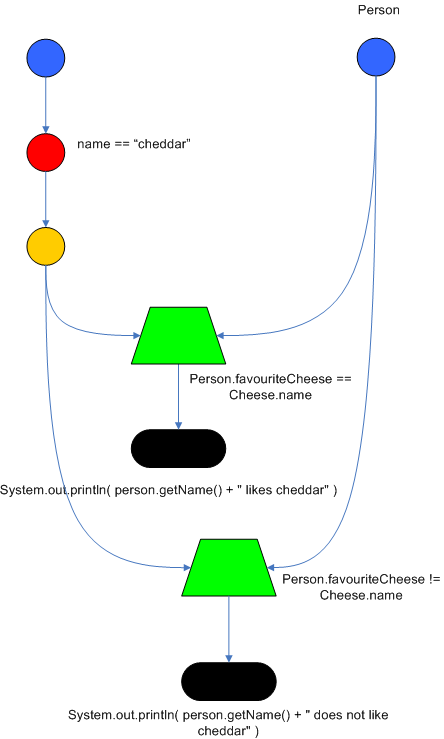
\includegraphics[width=12cm,height=12cm,keepaspectratio]{Pics/drools_rule_flow_example.png}
 			\caption{Esempio di flusso di valutazione di una regola Drools.}
 			\label{fig:DroolsRuleEvalFlow}
 		\end{center}
 	\end{figure}
 	
 	\hl{Nuova sottosezione: Spiegazione del flusso} \\
 	Un esempio di flusso di funzionamento è raffigurato nella \autoref{fig:DroolsRuleEvalFlow}. \\
 	In particolare i nodi azzurri sono degli \textit{ObjectTypeNode} e rappresentano nell'ordine formaggi e persone. \\
 	Il nodo rosso, invece, è di tipo \textit{AlphaNode} e verifica la condizione che il nome del formaggio sia "cheddar". \\
 	Il nodo giallo è di tipo \textit{LeftInputAdapterNode} e serve per scegliere dove dirottare il flusso a seguito del soddisfacimento o meno di una condizione prevista da un \textit{AlphaNode}.\\
 	Se la condizione prevista dall'\textit{AlphaNode} è verificata, il flusso viene inoltrato al primo punto di join (identificato da un trapezio verde) che verifica se il formaggio preferito dalla persona è il \textit{cheddar}. si dice punto di join perché per operare ha bisogno delle informazioni provenienti da due diverse entità gestite da degli \textit{ObjectTypeNode} distinti. \\ se la condizione prevista dall'\textit{AlphaNode} non è verificata, si passa al secondo punto di join.\\
 	In caso di verifica delle condizioni dei \textit{JoinNode}, si giunge ai nodi terminali ovvero al soddisfacimento delle condizioni che permette di prendere una decisione. In questo caso viene solo stampata una stringa, ma in generale è possibile scegliere l'azione più adatta al contesto di utilizzo.
 	
 	
 	\hl{Sistemare etichette dei nodi}

 	
 	
 	
 	
 	
 	
 	
 	
 	
 	
 	
 	
 	
 	
 	
 	
 	
 	
 	
 	
 	
 	
 	
 	
 	
 	
 	
 	
 	
 	
 	
 	
 	